%!TEX root = ./template-skripsi.tex
%-------------------------------------------------------------------------------
%                     BAB III
%               			PEMBAHASAN
%-------------------------------------------------------------------------------

\chapter{METODOLOGI PENELITIAN}

\section{Tahapan Penelitian}

Gambar \textit{flowchart} berikut mengilustrasikan proses pelatihan 
 dari dataset dan juga proses penggunaan yang sesungguhnya.

\begin{figure}[H]
  \centering{}
	\includegraphics[width=0.6\textwidth]{gambar/flowchart\_1\_1}
  \caption{Diagram alir untuk algoritma pelatihan klasifikasi objek}
\end{figure}

\begin{figure}[H]
  \centering{}
	\includegraphics[width=0.6\textwidth]{gambar/flowchart\_2}
  \caption{Diagram alir untuk algoritma pendeteksian objek}
\end{figure}

%(Jelasin disini secara ringkas, biar gak terlalu ambigu)

\section{Desain Sistem}

Dalam proses pembuatan \emph{classifier} perlu dilewati tahapan \textit{training}. 
Tujuan \textit{training} adalah untuk menciptakan suatu \emph{strong classifier} 
yang nantinya dapat digunakan untuk melakukan klasifikasi yang sebenarnya.
Pertama, gambar yang akan menjadi contoh pelatihan dianotasi sesuai kelasnya masing-masing dengan 
memberikan label yang sesuai dengan kelas mereka masing-masing, 
vontoh latihan ini berisikan gambar-gambar yang tidak memiliki kelas yang benar, atau 
\emph{false example} dan juga gambar-gambar yang memiliki kelas yang benar, atau 
\emph{positive example}. Setelah itu gambar melalui proses \emph{pre-processing} dan disesuaikan 
untuk mengoptimalkan proses pelatihan.

Pertama sebuah set \textit{features} akan dibuat dengan cara mencoba semua kemugnkinan 
yang ada dengan bentuk fitur yang dimiliki. Set ini akan berisikan informasi fitur-fitur 
yang nantinya akan dipakai untuk mendapatkan nilai fitur yang sesungguhnya. Set gambar latihan 
lalu akan dibaca menggunakan semua fitur ini dan hasilnya akan dicatat dalam tabel csv. 
Algoritma lalu akan mengkonstruksi sebuah \emph{decision tree} untuk setiap 
\emph{feature} untuk menentukan nilai \textit{feature threshold} setiap kelas. 
\emph{Decision tree} lalu akan di-\textit{boosting} untuk menentukan nilai bobot votingnya 
pada \textit{strong clossifier}. Akhrinya dari sekumpulan \emph{decision tree} ini dibuatlah 
sebuah \emph{final strong classifier} yang berbentuk \textit{cascade}.

Dengan \emph{final strong classifier}, barulah klasifikasi objek yang sesungguhnya dapat dilakukan. 
Pertama gambar yang akan dideteksi akan melalui \emph{pre-processing}. setiap sub-window akan dicek menggunakan 
\emph{strong classifier} untuk menentukan kelasnya. Hal ini dilakukan pada tiga area: area kiri untuk 
mengklasifikasi mulut dari ikan, area tengah untuk mengklasifikasi sirip dari ikan, dan terakhir area kanan 
untuk mengklasifikasi bentuk ekor dari ikan. Hasil ketiga \textit{sub-window} ini nantinya juga akan ber-\textit{voting}
dimana jika ada dua atau lebih \textit{sub window} berhasil mengklasifikasikan kelas yang sama, maka kelas itu 
dipilih sebagai kelas dari objek pada gambar. Kelas dari objek lalu akan dituliskan di pojok kiri atas gambar.

\section{Training \emph{Strong Classifier}}

Pada \textit{Training} ada tiga tahapan yang perlu dijalankan 
untuk menghasilkan sebuah \emph{Strong Classifier}, 
yaitu penginputan \textit{dataset} pelatihan yang sudah dianotasi, 
pembuatan \emph{features}, 
pembuatan \emph{decision tree} untuk setiap \emph{features}, 
\emph{Boosting }dan pemilihan fitur untuk pemebuatan \emph{attentional cascade}.

\subsection{\textit{Input Dataset} Pelatihan}

\begin{figure}[H]
  \centering{}
	\includegraphics[width=0.6\textwidth]{gambar/dataset\_2}
  \caption{Contoh gambar Abudefduf, Amphiprion, Chaetodon dan contoh gambar-gambar negatif}
\end{figure}

\textit{Dataset} yang akan dipakai diambil dari FishBase (Dapat dilihat di https://fishbase.mnhn.fr/) yang 
berisikan berbagai gambar ikan termasuk dari genus Abudefduf, Amphiprion dan Chaetodon. 
Ketiga genus ikan ini dipilih karena bentuknya yang berbeda satu-sama lain. Selain itu 
\textit{dataset} juga akan ditambahkan dari hasil penelitian lapangan 
secukupnya, dengan mempertimbangkan waktu komputasi pada tahap 
pelatihan.
Untuk contoh pelatihan gambar dibuat berukuran 350x200 piksel, 
dengan warna \textit{greyscale}. Selain itu juga akan dipilih contoh 
pelatihan negatif atau kumpulan gambar yang tidak terdapat kelas 
ikan dari http://www.vision.caltech.edu/datasets/ dengan jumlah yang sama, resolusi sama dan perlakuan 
yang sama. Anotasi dilakukan dengan menyimpan label dalam sebuah \textit{array}, label 
diambil dari sumber folder gambar. Kelas 0 direservasi untuk kelas negatif, sementara kelas 
1, 2 dan 3 direservasi untuk Abudefduf, Amphiprion dan Chaetodon.
\textit{Dataset} ini lalu dibagi menjadi tiga yaitu \textit{training dataset}, 
\textit{testing dataset}, dan \emph{validation dataset} dengan jumlah yang sama.

% \subsection{Pembuatan \textit{Integral Image}}

% Untuk pembuatan \emph{Integral Image}, pertama perlu dicari nilai piksel
% baris pertama dan kolom pertama dari gambar. Nilai pada matriks \emph{Integral Image} 
% adalah median dari nilai RGB pada piksel tersebut, namun dikarenakan warna 
% gambar sudah dirubah menjadi \emph{greyscale} maka nilai pada setiap piksel 
% hanya akan berupa bilangan bulat dikisaran 0 sampai 255. Nilai pada kolom 
% pertama hanyalah penjumlahan nilai piksel dari piksel $(0, 0)$ sampai ke piksel 
% $(0, j)$, sementara nilai pada baris pertama juga hanya penjumlahan nilai 
% piksel dari $(0, 0)$ ke  $(i, 0)$. Nilai-nilai piksel lainnya lalu dapat 
% dihitung menggunakan rumus: 
% \begin{equation}
%   \begin{split}
%     \text{integral image } (i,j) = {} & \text{integral image } (i-1,j) + \text{integral image } (i,j-1) - \\
%     & \text{integral image } (i-1,j-1) + \text{nilai dari piksel } (i,j)
%   \end{split}
% \end{equation}
% Atau jumlah semua nilai piksel dari $(0, 0)$ sampai ke $(i, j)$.
% Pembuatan \emph{integral image} nantinya akan digunakan oleh fitur sebagai \textit{input}.

% \begin{figure}[H]
%   \centering{}
% 	\includegraphics[width=0.6\textwidth]{gambar/integral\_image\_3}
%   \caption{Gambaran \emph{integral image} dari gambar sebuah bidak catur.}
% \end{figure}

\subsection{Pembuatan \textit{Haar like Features}}

Fitur-fitur yang akan digunakan dalam klasifikasi dibuat 
berdasarkan \emph{Haar-like Features} dan berisikan informasi penting yang dapat digunakan 
untuk mencari nilai sebuah fitur. Sebuah fitur berisikan tipe fiturnya, lokasi fitur tersebut 
didalam \textit{sub-window}, dan ukuran dari fitur tersebut.
Misalnya ada sebuah fitur, ia bertipe dua persegi menghadap ke kiri, lokasi x-nya adalah 12 piksel, 
dan lokasi y-nya adalah 10 piksel, dia memiliki ukuran 8 x 8 piksel.

\begin{figure}[H]
  \centering{}
	\includegraphics[width=0.6\textwidth]{gambar/feature\_data\_1}
  \caption{Sebuah fitur dua persegi menghadap ke kiri, lokasi x = 12 piksel, 
  lokasi y = 10 piksel, dengan ukuran 8 x 8 piksel.}
\end{figure} 
Dengan informasi yang ada didalam sebuah fitur tersebut, nilai fitur dapat dicari dengan 
mudah menggunakan rumus:

\begin{equation}
  \begin{split}
    \sum \text{nilai piksel area putih} -  \sum \text{nilai piksel area hitam} \\ 
  \end{split}
\end{equation}

Pada tahap ini fitur yang dipilih akan dibuat untuk semua 
posibilitas lokasi yang ada dan ukuran yang ada. Hal ini dilakukan dengan 
membuat fitur dimulai dari kiri atas gambar dengan ukuran 2 x 2 piksel untuk fitur 
dua persegi, empat persegi dan diagonal. Dan fitur 1 x 3 piksel atau 3 x 1 piksel untuk fitur tiga persegi, 
sampai pojok kanan bawah. Hal ini juga dilakukan sampai ukuran fitur lebih besar 
dari \emph{sub-window} tidak bisa muat lagi.

\subsection{Pembuatan \textit{Decision Tree}}

\begin{figure}[H]
  \centering{}
	\includegraphics[width=0.6\textwidth]{gambar/decision\_tree\_1}
  \caption{Contoh sebuah \textit{decision tree} dengan kelas 0, 1, 2 dan 3}
\end{figure} 

Setiap \emph{weak learner} adalah sebuah \emph{decision tree} yang akan mengambil nilai 
dengan fitur untuk digunakan sebagai variabel klasifikasi.
fitur dapat digunakan untuk mencari 
sebuah nilai perbandingan intensitas cahaya dari dua area pada gambar dan 
mendeteksi keberadaan suatu fitur seperti 
perbedaan warna, garis, maupun perbedaan kontras pada gambar.

\textit{Decision tree} pertama akan dibuat dari \textit{root} atau akar, yang lalu 
akan bercabang hingga batas maksimum telah dicapai. \textit{threshold} yang digunakan 
dalam pembuatan \textit{decision tree} adalah salah satu nilai fitur yang dibaca dari gambar. 
Dengan cara ini, \textit{decision tree} tidak perlu mencoba semua nilai yang mungkin, dan 
dengan demikian mempercepat proses pembuatan \textit{decision tree}.
Batas maksimum tinggi \textit{decision tree }yang dipilih adalah tiga 
tingkat, hal ini dikarenakan waktu komputasi yang memakan waktu bila \textit{decision tree} 
memiliki lebih dari 3 tingkat. Di lain sisi, menggunakan tingkat kurang dari tiga tidak mungkin 
memenuhi persyaratan klasifikasi empat kelas.

\subsection{\emph{Boosting}}

\emph{Boosting} ditunjukan untuk memberikan nilai \emph{voting} untuk setiap \textit{weak classifier} 
yang nantinya akan digunakan dalam klasifikasi akhir. Sebelum \emph{boosting} dimulai, 
\textit{weak classifier} yang kurang diskriminatif akan dibuang. Hal ini dilakukan dengan 
membandingkan hasil prediksi \textit{weak classifier} dengan label yang sebenarnya, dimana 
\textit{weak classifier} yang gagak memprediksi 50\% dari set tes akan dibuang. Ini dilakukan 
untuk mengurangi jumlah \textit{weak classifier} yang akan dipakai berikutnya.

Pada tahap ini \textit{boosting} 
akan dijalankan dari \textit{decision tree} yang paling akurat ke yang paling tidak akurat. Penentuan 
akurasi ini dilakukan dengan membandingkan label contoh validasi dengan hasil prediksi setiap \textit{weak classifier}. 
\textit{Weak classifier} yang tidak akurat akan mendapat suara \textit{voting} yang lemah. Rumus untuk mencari 
bobot voting \( \alpha \) dari sebuah \textit{weak classifier} adalah sebagai berikut:

\begin{equation}
  \begin{split}
    \epsilon = \frac{\sum_{i} \text{{image weights}}_i \times \text{{indikator}}_i}{\sum_{i} \text{{image weights}}_i} \\
   \alpha = 0.5 \times \log\left(\frac{1 - \epsilon}{\epsilon + 1e-10}\right) \\
  \end{split}
\end{equation}

\emph{weak classifier} terbaik akan mulai dan 
mengklasifikasi seluruh contoh \emph{dataset} validasi dan mencatat contoh yang 
gagal diklasifikasi oleh \emph{weak classifier} tersebut. Lalu bobot dari contoh tersebut akan 
dinaikan, dengan maksud agar bobot \textit{voting} fitur yang paling akurat akan lebih tinggi daripada 
fitur-fitur yang hanya mendekati menebak. Rumus menaikan bobot:

\begin{equation}
  \text{{image weights}} \times= \exp(\alpha \times \text{{indikator}})
\end{equation}
  
\begin{equation}
  \text{{image weights}} \div= \sum \text{{image weights}}
\end{equation}

\textit{weak classifier} berikutnya lalu akan melakukan prediksi dengan set yang sama, 
namun dengan bobot gambar yang sudah berubah karena \textit{weak classifier}. Sementara 
bobot \textit{voting weak classifier} sebelumnya akan disimpan ke array untuk digunakan nanti. 

Ketika semua \textit{weak learner} sudah dicari bobot \textit{voting}-nya, akan dibandingkan 
akurasi \textit{strong cloassifier} yang dibuat dengan iterasi sebelumnya. Bila didapat bahwa 
ada penurunan akurasi, maupun tidak ada perubahan, maka iterasi Boosting akan disudahi dan 
\textit{strong cloassifier} pada iterasi ini menjadi \textit{final strong classifier}.

\subsection{Pembuatan \emph{Attentional Cascade}}

\begin{figure}[H]
  \centering{}
	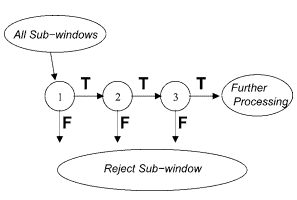
\includegraphics[width=0.6\textwidth]{gambar/cascade}
  \caption{\textit{Workflow} dari \emph{Attentional Cascade}}
\end{figure}

Karena bobot \textit{voting} dan urutan \textit{weak classifier} sudah ditentukan pada 
tahap \textit{Boosting}, pada tahap ini hanya perlu membagi \textit{weak classifier} menjadi 
beberapa \textit{stage} yang nantinya bisa dipanggil secara terpisah. Sebuah \textit{stage} 
berlaku layaknya sebuah \textit{strong cloassifier} kecil yang ditargetkan hanya memiliki 
tingkat akurasi paling tidak 50\% saja. Hal ini dilakukan agar pendeteksian seluruh \textit{sub-window} 
dapat dilakukan tanpa harus memanggil keseluruhan dari \textit{strong cloassifier}. 
Metode konstruksi sebuah \textit{stage cascade} adalah sebagai berikut:

\begin{algorithm}
  \caption{Cascade Train Stage}
  \begin{algorithmic}[1]
    \Function{Train\_stage}{}
      \State detection\_rate $\gets$ 0
      \While{detection\_rate $<$ 0.5}
        \If{$\text{len(features)} == 0$}
          \State \textbf{break}
        \EndIf
        \State self.features.append(features)

        \State detection\_rate $\gets$ accuracy\_score()
      \EndWhile
    \EndFunction
  \end{algorithmic}
\end{algorithm}

Sebelum pembuatan \emph{attentional cascade}, \emph{weaklearner} yang kurang 
diskriminatif akan dibuang dari \emph{Strong Classifier}. 
%Hal ini dilakukan dengan (cari, karena bagian ini 
%belum jelas dari kemarin). 
\emph{Attentional cascade} akan dibuat dari \emph{weaklearner} 
yang tersisa secara bertahap. 
Pertama, target \textit{false positive} pada setiap \emph{cascade} 
harus ditentukan oleh pengguna. \emph{Framework VIola-Jones} menggunakan target 
\textit{false positive} 50\% untuk \emph{cascade} pertama, dan 
\textit{false positive} 80\% untuk semua \emph{cascade} setelahnya.
Target \textit{false posiive} ini akan disesuaikan 
saat penelitian lapangan, bila target akurasi tidak berhasil dicapai 
dengan target \textit{false positive} sebelumnya.
Pada setiap fase \emph{cascade}, \emph{weaklearner} akan 
ditambahkan satu-persatu. Setiap sebuah \emph{weaklearner} ditambahkan, tes akan dilakukan 
dengan \emph{dataset} tes. \emph{Weaklearner} akan terus ditambahkan hingga \emph{false positive rate} 
yang ditentukan untuk fase itu dicapai. Fase akan terus bertambah hingga 
akurasi sempurna dicapai, atau hingga \emph{weaklearner} sudah habis. 
%(Ini periu dijabarin lagi dengan rumus per-step). 


\section{Skenario Eksperimen dan Validasi}

Tahapan ini adalah penggunakaan \emph{classifier} yang sebenarnya dengan tujuan 
memvalidasi akurasi dari \emph{classifier} tersebut. 
Gambar ikan yang akan dipakai dalam proses validasi akan 
melalui beberapa langkah dalam tahap ini, 
yaitu: \textit{Pre-processing} dalam bentuk \emph{grayscaling}, Penghitungan 
\emph{Integral Image}, dan deteksi yang sesungguhnya menggunakan \emph{strong classsifier} 
yang telah dibuat dengan metode Sliding Window.

\subsection{\textit{Pre-processing} dan Penghitungan \emph{Integral Image}}

Untuk klasifikasi sebenarnya, gambar \emph{input} akan diproses terlebih dahulu. 
Gambar awalnya akan melakui proses \textit{pre-processing} dan dirubah kedalam warna 
\emph{grayscale} %(Jelasin perubahan greyscale ini kayak gimana) 
untuk mempermudah penghitungan dengan bantuan \emph{library OpenCV}. 
Setelah tu sebuah matriks sebesar resolusi gambar akan dibuat untuk 
penghitungan \emph{Integral Image} yang nantinya akan mempercepat proses 
penghitungan fitur. Pembuatan \emph{integral image} pada tahap ini sama persis 
dengan pembuatan pada tahap pelatihan.

\subsection{Klasifikasi}

Pada tahap ini, gambar yang sudah berubah dalam bentuk 
\emph{integral image} akan diklasifikasi menggunakan 
\emph{strong classifier}. \emph{Strong classifier} akan berjalan dari 
pojok kiri atas gambar, atau piksel pertama, mencoba untuk mengklasifikasi 
sebuah \emph{sub-window} berukuran 72x41 piksel. Bila posisi tersebut sudah 
selesai diklasifikasi, terlepas hasilnya, \emph{sub-window} akan 
bergerak ke kanan sebanyak satu piksel dan mengklasifikasi area baru tersebut. 
Hal ini akan terus berlanjut hingga \emph{sub-window} bisa dibuat lagi ke kanan. 
Bilama demikian \emph{sub-window} akan kembali ke ka kanan, namun kali ini 
diturunkan sebanyak satu piksel. Pergerakan \emph{sliding window} ini 
bertujuan agar seluruh bagian dari gambar dapat terklasifikasi.

\begin{figure}[H]
  \centering{}
	\includegraphics[width=0.6\textwidth]{gambar/sliding\_window\_1}
  \caption{Gambaran ukuran \emph{sub-window} 72x41 piksel pada gambar 300x220}
\end{figure}

Jika \emph{sub-window} dengan ukuran 72x42 piksel sudah mengklasifikasi 
seluruh bagian gambar hingga pojok kanan bawah, maka \emph{sub-window} 
akan diperbesar dengan faktor 1.25 dan proses dimulai lagi dari pojok kiri atas. 
Selain itu ukuran dan lokasi dari \emph{feature} akan disesuaikan untuk mangakomodasi 
\emph{sub-window} yang sudah diperbesar. Hal ini dilakukan untuk mengklasifikasi 
objek yang memiliki ukuran berbeda didalam gambar.

\subsection{Anotasi}

\begin{figure}[H]
  \centering{}
	\includegraphics[width=0.6\textwidth]{gambar/sliding\_window\_2}
  \caption{Gambaran \textit{sub-window} yang berhasil mengklasifikasi ikan didalam gambar}
\end{figure}

Setelah semua \textit{sub-window} sudah diklasifikasi dengan menggunakan 
\emph{strong classifier}. Algoritma akan menggambarkan di lokasi \textit{sub-window} 
yang positif terklasifikasi (Memiliki salah satu kelas ikan yang telah dilatih ke \emph{strong classifier}), 
\emph{bounding box} untuk menganotasi kelasnya. Pengguna lalu dapat menentukan 
dari hasil anotasi bilamana target akurasi sudah tercapai.


